\documentclass{beamer}
\usepackage{amssymb,amsmath,amsfonts,pdfpages,color, url}
\usepackage{booktabs}
\usepackage{wrapfig}
\usepackage{amsmath}
\usepackage{multirow}

\setbeamertemplate{navigation symbols}{}
\usetheme{Montpellier}

\setbeamertemplate{footline}[page number]


\def\dis{\mathop{\displaystyle}}
\def\argmin{\mathop{\rm argmin}}


\newcommand{\E}{\mathbb{E}}
\newcommand{\jeff}[1]{{\color{blue}$\langle$Jeff: #1$\rangle$}}
\newcommand{\dgen}{\ensuremath{\mathtt{d}}}



\title{Efficient Trajectory Retrieval}
\author{Hasan Pourmahmood}
%\date{}

\begin{document}

\frame{\titlepage}


\section{Motivation}

\begin{frame} 
\frametitle{Trajectory}
\begin{block}{}
A spatial trajectory (also called a piece-wise linear curve) is a sequence of waypoints along with a time stamp, i.e. 
$$T=\{(x_1, y_1, t_1), \ldots, (x_n, y_n, t_n)\}.$$
\begin{figure}[h] 
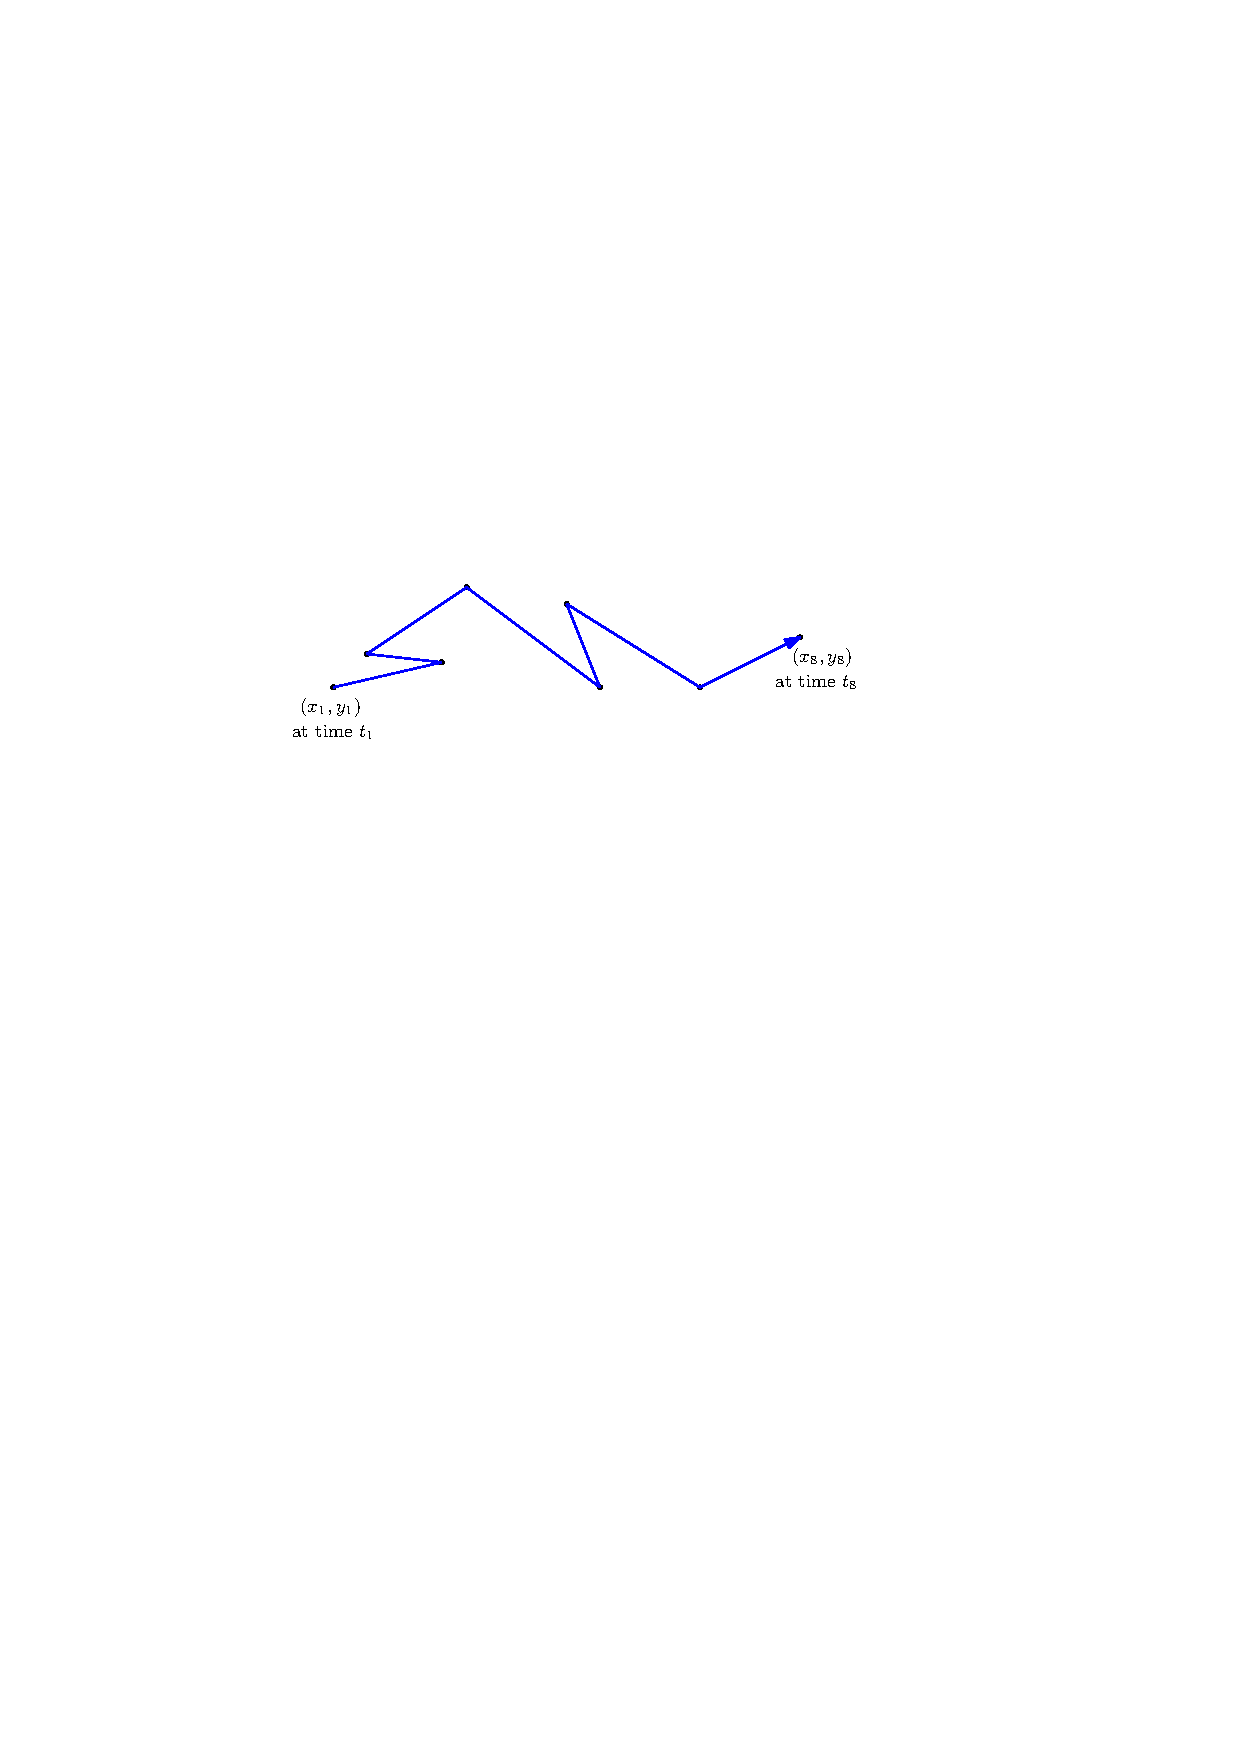
\includegraphics[width=0.8 \textwidth]{trajectory} 
\end{figure}  \vspace{-1mm}
\end{block} 
\end{frame}




\begin{frame}
\frametitle{}
\begin{block}{Popular Distances}
\begin{itemize}
\item [$\blacktriangleright$] Dynamic Time Warping distance 

\item [$\blacktriangleright$] Fr\'echet distance 

\item [$\blacktriangleright$] Discrete Fr\'echet distance \pause 
\end{itemize}
Complexity: {\color{orange} Quadratic in number of waypoints $O(mn)$}.
\end{block} \pause

\begin{block}{Queryies}
\begin{itemize}
\item {\color{blue} $k$-NN queries:} find $k$ nearest trajectories from data to the given query trajectory $Q$.
\item {\color{blue} Range queries:} find all trajectories within distance $r$ from data to the given query trajectory $Q$.
\end{itemize}
\end{block} \pause

\begin{block}{Applications}
{\small Route extraction, route recommendation, ML on trajectory datasets, ...}
\end{block}
\end{frame}


\section{Information Retrieval}

\begin{frame}
\frametitle{Information retrieval approach} \pause
\begin{block}{Treating the problem as a ``term-document" pair}
\begin{itemize} \pause
\item Consider a grid structure with some resolution for the region {\color{blue} $R$}, where data lives in, in order to get term-document representation. Each grid will be treated as a term. \pause
\item Map each trajectory (as a document) to a vector space of large but fixed dimension. \pause
\item Employ a dimensionality reduction technique to reduce the dimension (our {\color{blue} index}). \pause
\item Utilizing this vector space model in a lower dimensional space, consider a similarity measure between reduced vectors. \pause
\item Answer to the queries in an efficient way.
\end{itemize}
\end{block}
\end{frame}



\begin{frame}
\frametitle{Experiments, Evaluation and Interface} \pause
\begin{block}{}
\begin{itemize} 
\item Consider 2 or 3 real world trajectory data sets. \pause
\item Use the vector space model on data sets and evaluate the performance of the search method using all data points as queries. \pause
\item Report some statistics like {\color{blue} accuracy, precision, recall, nDCG}. \pause
\item Provide an interactive {\color{blue} user-friendly interface} for arbitrary queries on the map, where a user can create a query trajectory by clicking on the map and specifying the value of $k$ (or $r$) to get the the recommended $k$ nearest trajectories from data on the map visually.  
\end{itemize}
\end{block}
\end{frame}



\begin{frame}
\frametitle{My contributions} \pause
\begin{block}{}
\begin{enumerate} 
\item Using different datasets as benchmark, \pause
\item Utlizing binary vectorization of trajectories, \pause
\item Using term-frequency type of trajectory vectorization, \pause
\item Using a landmark-based vectorization (if time allows), \pause
%\item Applying different dimensionality reduction techniques, \pause
\item Employing a kernel-based similarity measure for terms, \pause
\item In addition to the metric used in the reference paper, I will try to apply DTW or discrete Fr\'echet distance as a ground truth, \pause
\item Providing a user-friendly interactive visualization tool for retrieving target trajectories. 
\end{enumerate}

\end{block}
\end{frame}




\section*{Questions/Comments}
{\color{white}1}
\begin{center} 
{\huge \color{magenta}{\sc \vspace{3cm} Questions/Comments?}}
\end{center}


































\end{document}